\chapter [Introdução]{Introdução}

\section{Contextualização}

% Falar sobre a importância das energias renováveis no contexto mundial

A crescente demanda de energia e a urgente atenção para causas ambientais exigem sistemas de energia eficientes e ecológicos. 
As energias renováveis são consideradas como alternativas promissoras para os sistemas convencionais de combustíveis fósseis, adotados em peso ao redor do mundo, e portanto, tem chamado cada vez mais atenção \cite{Guo2018}.
A Fig. \ref{fig:energy-resources} mostra o potencial que as energias renováveis tem de fornecer até mais de 3000 vezes a demanda atual de energia.

\begin{figure}[!hbt]
	\begin{center}
    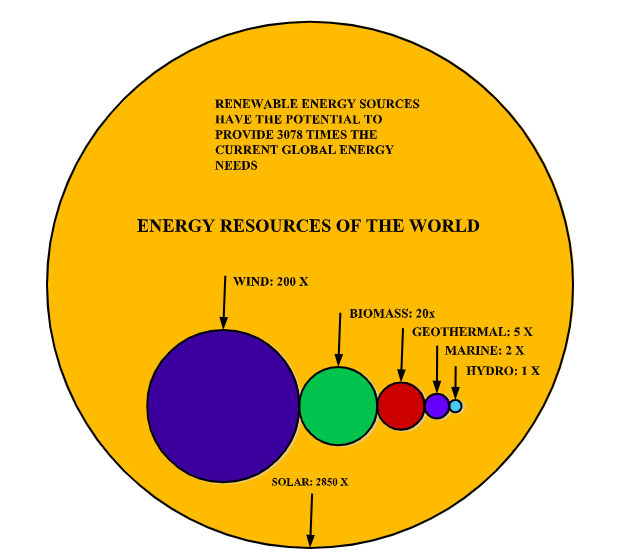
\includegraphics[width=0.5\textwidth]{figuras/Energy_Resources_of_The_World.png}
    \caption{Recursos de energia no mundo. Fonte: \cite{Ellabban2014}}
    \label{fig:energy-resources}
    \end{center}
\end{figure}

A IEA (\textit{International Energy Agency}) possui o WEO (\textit{World Energy Outlook}), que é 
um padrão de análise de energia a longo prazo. 

A edição do ano de 2018 deste padrão 
forneceu análises atualizadas de dados recentes, tendências de tecnologia e anúncios de políticas 
que podem ser significativas para o setor de energia até o ano de 2040.

O WEO 2018 detalhou as tendências globais de energia e qual o possível impacto que elas terão sobre 
a oferta e a demanda, as emissões de carbono, a poluição do ar e o acesso à energia. 

Foi feita uma análise baseada em cenários que descreveu diferentes futuros 
para o sistema energético, contrastando o caminho adotado pelas políticas atuais e planejadas 
com as que podem atender às metas climáticas de longo prazo do Acordo de Paris \footnote{Na 21ª 
Conferência das Partes (COP21) da UNFCCC, em Paris, foi adotado um novo acordo com o objetivo 
central de fortalecer a resposta global à ameaça da mudança do clima e de reforçar a capacidade dos 
países para lidar com os impactos decorrentes dessas mudanças. O Acordo de Paris foi aprovado pelos 
195 países partes da UNFCCC para reduzir emissões de gases de efeito estufa (GEE) no contexto do 
desenvolvimento sustentável \cite{MME}.}, reduzir a poluição do ar e garantir o acesso universal à energia.

As análises realizadas pelo WEO 2018 demonstraram que os governos terão uma influência crítica na 
direção do futuro sistema energético mundial. Com base nos acordos políticos mundiais atuais e nos 
planejados, é possível modelar como será o futuro da utilização das fontes de energia e a 
utilização das energias renováveis no mundo. 
O WEO realizou este modelamento no cenário conhecido como \textit{\textbf{New Policies Scenario}}, 
que demonstrou que a demanda mundial de energia deve crescer mais de 25\% até 2040, exigindo mais de US\$ 2 trilhões por ano de investimento em novos suprimentos de energia \cite{WEO2018}.

O uso das energias renováveis teve um forte crescimento nos últimos anos, principalmente nos setores
especializados na produção de energia elétrica, mas a adoção destas 
tem sido mais lenta na indústria, nos edifícios e nos transportes.
Algumas tecnologias de energias renováveis, como a energia solar fotovoltaica e a 
eólica \textit{onshore}, estão adquirindo competitividade; outras, como a 
energia eólica \textit{offshore}, estão equilibradas entre a necessidade de apoio e a 
competitividade, enquanto tecnologias como a energia das marés e ondas 
ainda precisam de suporte \cite{WEO2018}.

A Fig. \ref{fig:geracao-capacidade-energias-renovaveis} mostra uma perspectiva da geração e capacidade 
das energias renováveis ao redor do mundo utilizando o \textit{New Policies Scenario}. 
É possível ver que a geração de eletricidade a partir de fontes renováveis quase 
triplica até 2040 e representa mais de 40\% da geração geral.
Há um crescimento no uso direto de fontes renováveis em aplicações de transporte e aquecimento, 
mas a participação destes setores é menor.
A utilização das energias renováveis no aquecimento de casas e edifícios aumenta neste 
cenário em cinco pontos percentuais, para 15 \% em 2040.
Espera-se que cerca de 60\% desse aumento ocorra na China, União Europeia, Índia e Estados Unidos, 
que são hoje os maiores consumidores de sistemas de calefação à base de energias renováveis.
Nos transportes, a parcela de energias renováveis mais que dobra, atingindo cerca de 8\%. 
Prevê-se que a demanda por biocombustíveis aumente para 4,7 mboe/d, representando 6\% do uso 
de energias renováveis no transporte em 2040 \cite{WEO2018}.

\begin{figure}[!hbt]
	\begin{center}
    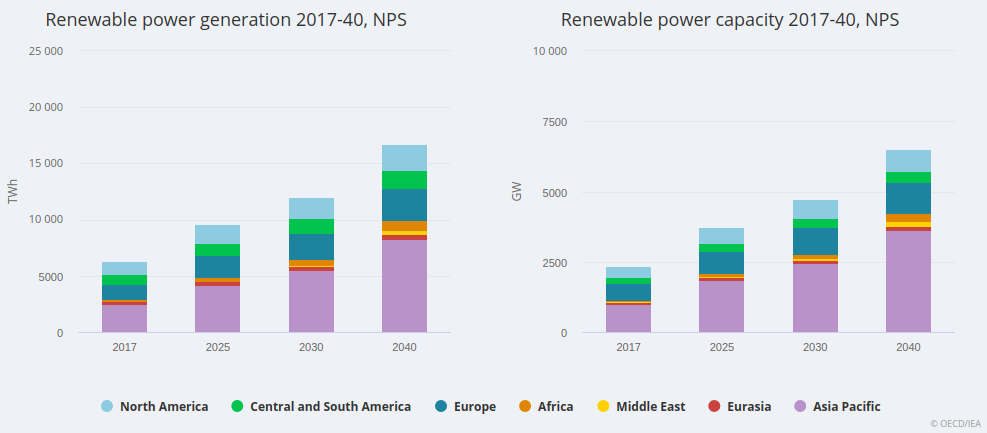
\includegraphics[width=\textwidth]{figuras/geracao_capacidade_potencia_energias_renovaveis.png}
    \caption{Perspectiva da geração de energia e capacidade de potência com a utilização de energias renováveis de 2017 à 2040. Fonte: \cite{WEO2018}}
    \label{fig:geracao-capacidade-energias-renovaveis}
    \end{center}
\end{figure}

As mudanças climáticas e a poluição do ar estão entre os principais fatores que estimulam o 
emprego de fontes renováveis no mundo. 
A poluição do ar é o principal fator em países como China e Índia. 
Na Europa, há uma atenção crescente aos efeitos nocivos à saúde da poluição atmosférica, amplamente relacionados ao fornecimento e uso de energia \cite{Gielen2019}.

% Falar sobre a utilizacao, crescimento e perspectivas da utilização da energia eólica no contexto mundial

Nos últimos 30 anos, os sistemas envolvendo energia solar e eólica vem melhorando suas 
características de desempenho e experimentado um rápido crescimento de vendas. 
De fato, a energia eólica parece ter uma vantagem maior, pois pode ser empregada em 
larga escala a um custo razoável, ainda que em comparação com outras fontes \cite{Kumar2016}.

Segundo a WWEA (\textit{World Wind Energy Association}), a capacidade mundial de potência 
usando energia eólica atingiu 597 GW, com um adição de 50,1 GW em 2018.
O ano de 2018 foi o segundo ano consecutivo com um número crescente de novas instalações, 
mas com uma taxa de crescimento menor de 9,1\%. Para fins de comparação, no ano de 2017 houve uma 
taxa de crescimento de 10,8\%.
Todas as turbinas eólicas instaladas até o final de 2018 podem cobrir cerca de 6\% da demanda global de eletricidade.

A Tab. \ref{tab:capacidade-instalada} mostra um comparativo da capacidade instalada de unidades eólicas entre os anos de 2015 e 2018 entre vários países.
Verifica-se que os maiores líderes de mercado são a China e os EUA, tendo o Brasil um papel de destaque no comparativo mundial \cite{WEI}.

\begin{table}[h]
	\centering
	\caption{Capacidade das instalações eólicas até o final de 2018 (MW). Fonte: \cite{WEI}}
	\label{tab:capacidade-instalada}
	
	\begin{tabular}{ccccc}
		\toprule
		\textbf{País/Região} & \textbf{2018} & \textbf{2017} & \textbf{2016} & \textbf{2015}\\
		\midrule
		China & 216.870 & 195.730 & 168.730 & 148.000 \\
		Estados Unidos & 96.363 & 88.775 & 82.033 & 73.867 \\
		Alemanha & 59.313 & 56.190 & 50.019 & 45.192 \\
		Índia & 35.017 & 32.879 & 28.279 & 24.759 \\
		Espanha & 23.494 & 23.026 & 23.020 & 22.987 \\
		Reino Unido & 20.743 & 17.852 & 14.512 & 13.614 \\
		França & 15.313 & 13.760 & 12.065 & 10.293 \\
        Brasil & 14.490 & 12.763 & 10.800 & 8.715 \\
        Canadá & 12.816 & 12.239 & 11.898 & 11.205 \\
        Resto do mundo & 102.138 & 93.173 & 85.582 & 76.653 \\
        \textbf{Total geral} & \textbf{596.556} & \textbf{546.388} & \textbf{486.939} & \textbf{435.284} \\
		\bottomrule
	\end{tabular}
\end{table}

% Comentar sobre a matriz energética atual brasileira

O Brasil possui um potencial eólio-elétrico estimado 
pelo Atlas do Potencial Eólico Brasileiro de 143 GW e isto se deve principalmente
por conta de sua extensão territorial, por suas extensas planícies e relevos, 
assim como climas que se diversificam entre quentes e úmidos que colaboram para a ocorrência 
de ventos fortes - velocidades médias anuais de até 8,5 m/s em estados do Nordeste e 
acima de 7 m/s no Rio Grande do Sul - 
regulares e de grande estabilidade em sua direção \cite{Pinto2019},.

A Fig. \ref{fig:matriz-energetica-brasileira} apresenta a matriz energética brasileira e mostra que a energia eólica já é a segunda maior fonte de energia elétrica da matriz. 
De fato, no final de 2017, a participação destas era de 8,1\%, saltando para 9,0\% em 2019, mostrando o crescimento e a relevância desta fonte de energia no âmbito nacional \cite{ABEeolica}.

% Falar sobre a utilização, crescimento e perspectivas da utilização da energia eólica no cenário brasileiro

\begin{figure}[!hbt]
	\begin{center}
    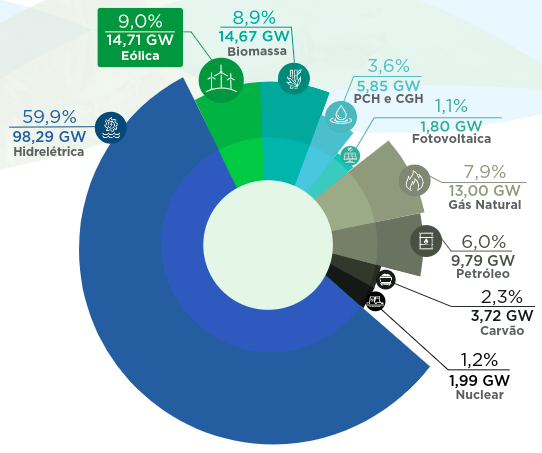
\includegraphics[width=0.5\textwidth]{figuras/matriz_eletrica_brasileira.png}
    \caption{Matriz Energética Brasileira (GW). Fonte: \cite{ABEeolica}}
    \label{fig:matriz-energetica-brasileira}
    \end{center}
\end{figure}

\section{Descrição do Problema}

% Comentar sobre as normas e regulamentos que regem a utilização da energia eólica no mundo e no Brasil
% Comentar sobre a utilização e projetos de conversores eletrônicos de potência
% Fazer um parágrafo relacionionando o projeto de conversores eletrônicos com a proposta apresentada no presente trabalho

Nos sistemas de geração de energia eólica, os conversores eletrônicos de potência são predominantemente 
aplicados para regular a energia flutuante de entrada e maximizar a energia elétrica colhida do 
vento \cite{Ellabban2014}.

A operação de um sistema eólico é definida pelas características dinâmicas do vento e da turbina e a 
atuação dos dispositivos de eletrônica de potência.
Desta forma, o acoplamento entre unidades eólicas e a rede básica de energia elétrica pode levar a 
pertubações nas tensões e correntes do sistema \cite{TeseProfAlex}.

Consequentemente, a Qualidade de Energia Elétrica (QEE) torna-se um ponto relevante, 
pois é necessário atender requisitos estabelecidos por normas, 
recomendações técnicas específicas e códigos de rede de cada país para assegurar 
uma adequada integração das centrais eolicas à rede \cite{DissertacaoJoao}.

No Brasil, o ONS (Operador Nacional do Sistema) é responsável, dentro de suas atribuições, por realizar o controle de desempenho da rede básica do SIN (Sistema Interligado Nacional).
Exemplos de indicadores que devem ser monitorados são: a conformidade da forma de onda, dentre estes a distorção harmônica, o desequilíbrio e flutuação de tensão \cite{DissertacaoLeandro}.

Dentro do contexto de qualidade de energia elétrica, a regulamentação vigente exige a realização de estudos computacionais e de medições para aceitação de novos acessos de parques eólicos. 
Os estudos são necessários para avaliação de condições problemáticas de conexão entre os empreendimentos eólicos e o sistema elétrico, problemas que podem ter origem tanto no interior dos parques eólicos quanto na rede de conexão \cite{DissertacaoLeandro}.

Baseado na motivação e na problemática apresentadas, o presente trabalho visa apresentar uma proposta 
de bancada para estudos de desempenho de unidades eólicas através do projeto de um inversor 
trifásico \textit{half-bridge} com a utilização de um modelo computacional apoiado no uso de simulações
para validação da teoria apresentada e dos resultados teóricos de projeto do inversor, e a comprovação 
do funcionamento do protótipo através de testes laboratoriais.

\section{Objetivos}

\subsection{Objetivo Geral}
O presente trabalho tem por objetivo a montagem de uma bancada laboratorial para estudos de conexão de unidades eólicas às redes elétricas, sendo constituída por
um inversor trifásico de três braços, filtros de acoplamento, sistema de aquisição de dados e DSP da Texas Instruments TMS320F28335.

\subsection{Objetivos Específicos}
De forma a atender o objetivo em questão, propõe-se:
\begin{itemize}
        \item Estudar as técnicas de controle de inversores trifásicos, metodologias de sincronismo, filtros de conexão à rede elétrica;
        \item Realizar simulações computacionais para validação do modelo teórico;
        \item Realizar as montagens experimentais e validar o funcionamento dos controladores.
\end{itemize}

\section{Organização do Trabalho}

Para apresentação e consolidação dos objetivos propostos, o presente trabalho está organizado da seguinte forma:

\begin{itemize}
	\item Capítulo 2 - Fundamentação Teórica: Objetiva consolidar os conceitos teóricos necessários para a compreensão das metodologias apresentadas no trabalho.
	\item Capítulo 3 - Metodologia: Visa apresentar os componentes laboratoriais utilizados, sua organização e disposição para atingir os objetivos propostos. Demonstra os procedimentos utilizados para obtenção dos resultados de simulação computacionais e experimentais.
	\item Capítulo 4 - Resultados e Discussões: Objetiva mostrar os dados de simulação e experimentais obtidos utilizando as metodologias propostas através de gráficos e tabelas. Neste capítulo, os resultados de simulação e experimentais são comparados para atestar o funcionamento correto da bancada.
	\item Capítulo 5 - Conclusões: Propõe-se a retomar os resultados discutidos com os objetivos propostos e comentar sobre futuras aplicações do protótipo desenvolvido para estudos envolvendo sistemas eólicos.
\end{itemize}